\begin{figure}[!ht]
\centering
\begin{tabular}{c@{\hskip 7ex}c}

 %%%%%%%%%%%%%%%%%%%%%%%%%%%%%% P_U^{ER}+P_U^{DR} wsj_1818%%%%%%%%%%%%%%%%%%%%%%
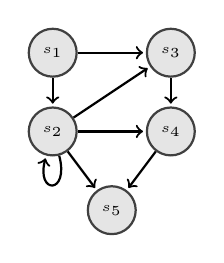
\begin{tikzpicture}[shorten >=1pt,->,scale=0.5]  
        \tikzstyle{sentence}=[circle,thick,draw=black!75,fill=black!10,minimum size=2mm]
        \tikzstyle{edge}=[draw, thick]
       \begin{scope}
         \node [sentence] (s1) at (0,4) {\tiny{$s_1$}};
         \node [sentence] (s2) at (0,2) {\tiny{$s_2$}};
         \node [sentence] (s3) at (3,4) {\tiny{$s_3$}}; 
         \node [sentence] (s4) at (3,2) {\tiny{$s_4$}}; 
         \node [sentence] (s5) at (1.5,0) {\tiny{$s_5$}}; 

         \path[edge] (s1) edge [above] node[font=\tiny] {} (s2);
         \path[edge] (s2) edge [above] node[font=\tiny] {} (s3);
         \path[edge, loop below] (s2) edge [above] node[font=\tiny] {} (s2);
         \path[edge] (s3) edge [above] node[font=\tiny] {} (s4);
         \path[edge] (s4) edge [above] node[font=\tiny] {} (s5);
         
         \path[edge] (s1) edge [above] node[font=\tiny]{} (s3);
 		\path[edge] (s2) edge [above] node[font=\tiny]{} (s4);
		\path[edge] (s2) edge [above] node[font=\tiny]{} (s5);
% 		\path[edge] (s4) edge [above] node[font=\tiny]{} (s5);
        \end{scope}        
      \end{tikzpicture}
&
%%%%%%%%%%%%%%%%%%%%%%%%%%%%%%  P_w^{DR} wsj_1818%%%%%%%%%%%%%%%%%%%%%%
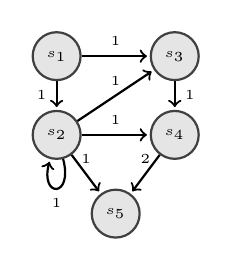
\begin{tikzpicture}[shorten >=1pt,->,scale=0.5]  
        \tikzstyle{sentence}=[circle,thick,draw=black!75,fill=black!10,minimum size=2mm]
        \tikzstyle{edge}=[draw, thick]
       \begin{scope}
         \node [sentence] (s1) at (0,4) {\tiny{$s_1$}};
         \node [sentence] (s2) at (0,2) {\tiny{$s_2$}};
         \node [sentence] (s3) at (3,4) {\tiny{$s_3$}}; 
         \node [sentence] (s4) at (3,2) {\tiny{$s_4$}}; 
         \node [sentence] (s5) at (1.5,0) {\tiny{$s_5$}}; 

         \path[edge] (s1) edge [left] node[font=\tiny] {$1$} (s2);
         \path[edge] (s2) edge [above] node[font=\tiny] {$1$} (s3);
         \path[edge, loop below] (s2) edge [below] node[font=\tiny] {$1$} (s2);
         \path[edge] (s3) edge [right] node[font=\tiny] {$1$} (s4);
         \path[edge] (s4) edge [above] node[font=\tiny] {$2$} (s5);
         
    		\path[edge] (s1) edge [above] node[font=\tiny]{1} (s3);
 		\path[edge] (s2) edge [above] node[font=\tiny]{1} (s4);
		\path[edge] (s2) edge [above] node[font=\tiny]{1} (s5);
% 		\path[edge] (s4) edge [above] node[font=\tiny]{1} (s5);
        \end{scope}        
      \end{tikzpicture}

 
\\

\scriptsize{$P_u^{ER} \lor P_u^{DR}$} & \scriptsize{$P_w^{ER} + P_w^{DR}$} 
                 

\end{tabular}
\caption{Combined entity and discourse relation graphs.}
\label{f:combined_graphs}
\end{figure}